\section{2024年11月29日} % 日期作为章节显示在目录中

\subsection{今日进展} % 今日进展
1. 禁手规则判断:

   - 实现了五子棋的禁手规则检测,包括四种禁手类型:三三禁手、四四禁手、四三禁手和长连禁手。通过检测棋盘上的活三、活四和长连等棋型,成功防止了 AI 进行禁手操作。

2. 局面评估功能:

   - 完成了初步的局面评估功能,结合禁手规则,能够根据当前棋局对每个落子进行评分,评估玩家的进攻和防守局面。

3. 菜单功能:

   - 实现了一个简单的游戏菜单,允许玩家设置黑棋(X)和白棋(O)的玩家类型(人类或 AI)。通过菜单,玩家可以选择是否开始游戏或退出程序。

4. AI 随机算法:

   - 为 AI 实现了一个简单的随机落子算法,使得 AI 能够在棋盘上随机选择一个空位置进行落子。

5. 输入函数设计:

   - 设计并实现了一个输入函数,方便了后续 AI 模块的接入。输入函数根据玩家类型(人类或 AI)动态选择适当的输入方式,简化了 AI 和人类玩家之间的交互。

\subsection{成果展示} % 成果展示

\subsubsection{程序界面截图}
\begin{figure}[h]
    \centering
    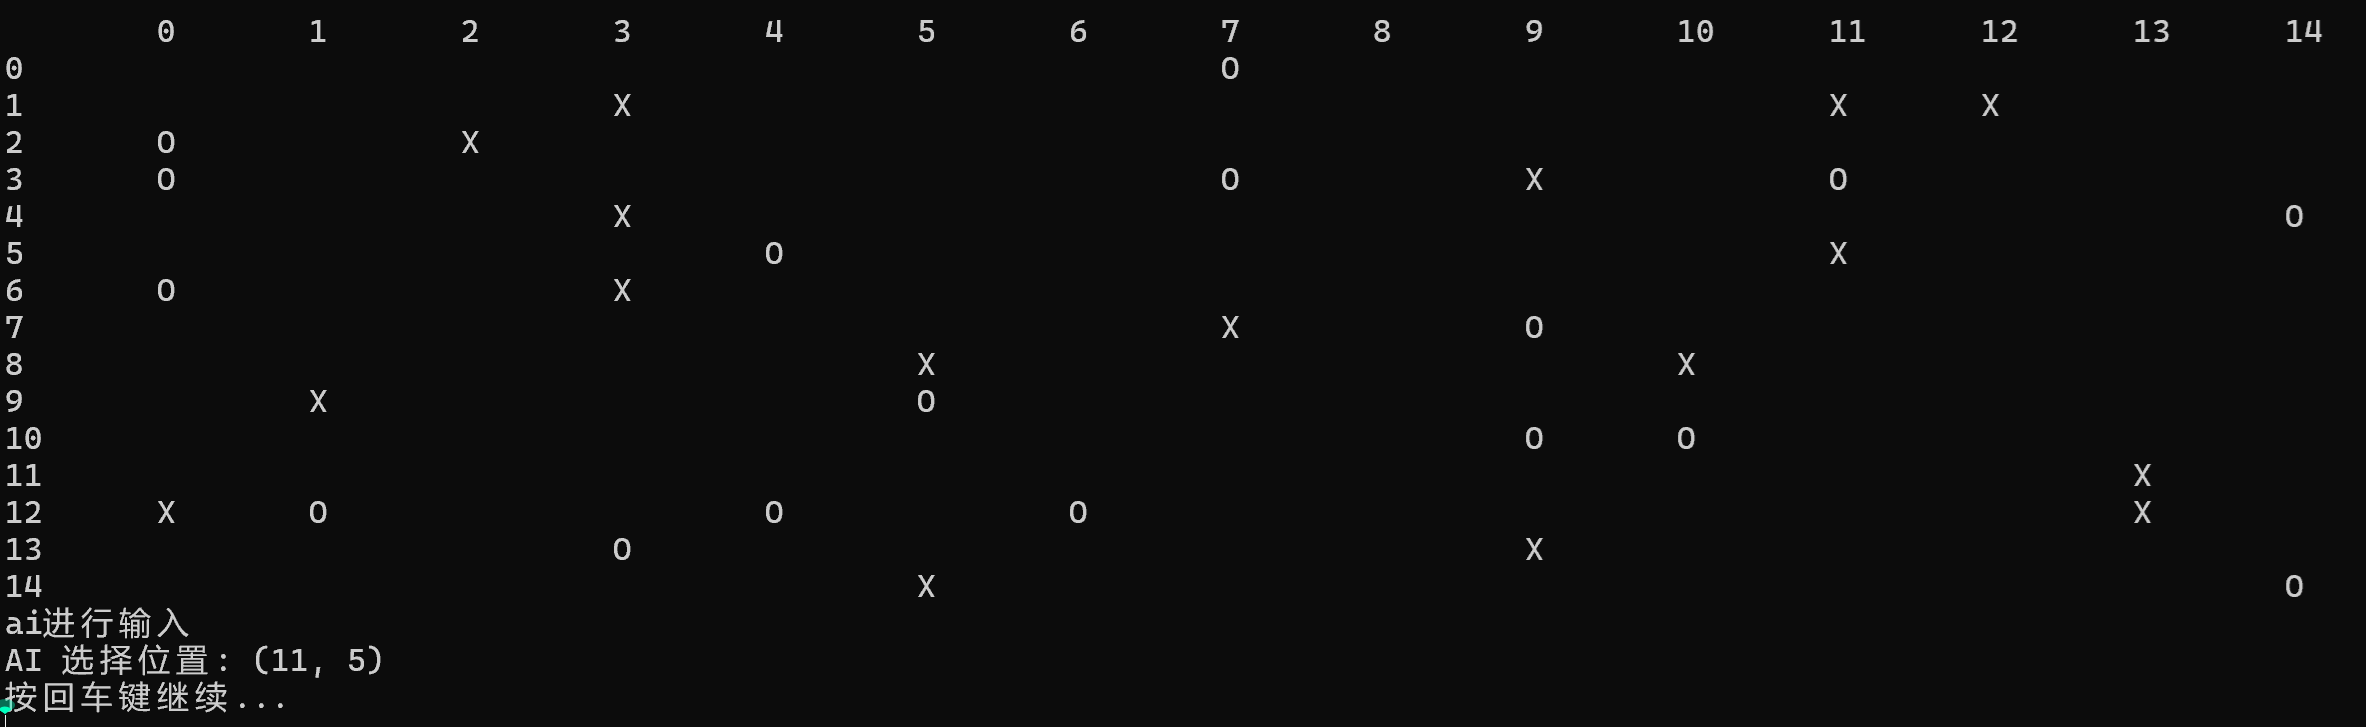
\includegraphics[width=0.7\textwidth]{logs/image/29日界面.png}
    \caption{AI自我对弈运行截图}
    \label{fig:program_output}
\end{figure}

\subsubsection{运行结果}
1. 禁手规则检测功能成功运行,能够在 AI 落子时避免三三禁手、四四禁手等情况。

2. 随机 AI 在每轮对局中能够随机选择空位置进行落子,且避免禁手操作。

3. 游戏菜单能够正常运行,玩家能够选择黑棋和白棋的玩家类型,并选择开始游戏或退出程序。

4. 目前,AI 和玩家在同一个棋盘上交替落子,程序能够判断胜负、平局以及禁手,确保游戏规则正常执行。

5. 输入函数已成功集成,允许根据玩家类型选择合适的输入方式,便于后续 AI 模块的接入。

\subsection{问题与解决方案} % 问题与解决方案

\subsubsection{遇到的问题}
1. 禁手规则判断存在逻辑漏洞:

   - 初期禁手规则检测时,发现没有正确处理一些复杂局面,尤其是四四禁手和三三禁手的检测,导致 AI 在某些情况下可能仍会选择禁手棋步。
   
2. AI 决策过于简单:

   - 当前的 AI 只使用随机算法选择棋步,虽然可以避免禁手,但缺乏战略性,导致游戏体验较为简单,缺乏挑战性。

3. 棋盘显示与用户交互较为简单:

   - 当前的程序仅依赖终端输出,缺少图形化界面,用户体验较差。

\subsubsection{解决方法}
1. 禁手规则优化:

   - 对三三禁手和四四禁手的判断进行了优化。通过细化禁手检测函数,增加了对活三和活四的严格检查,确保 AI 在选择棋步时能够避开这些禁手规则。
   
2. AI 改进:

   - 目前的 AI 仍然依赖随机算法,下一步将实现基于局面评估函数的 Minimax 算法,并结合 Alpha-Beta 剪枝提升 AI 的智能程度。

3. 游戏菜单优化:

   - 完成了游戏菜单功能,能够实现玩家与 AI 之间的设置。接下来会考虑实现简单的图形界面,以提高用户体验,使游戏界面更加直观。

4. 输入函数集成:

   - 设计并实现了一个简洁的输入函数,解决了不同玩家类型(人类或 AI)之间的输入方式问题。这个函数简化了后续 AI 模块的接入,使得系统更加灵活。

\subsection{代码分析} % 代码分析

\subsubsection{禁手规则检测代码}
\begin{lstlisting}[caption={禁手规则判断核心代码}, label={code:forbiddenMove}]
bool isForbiddenMove(const vector<vector<char>>& board, int x, int y) 
{
    int liveThreeCount = 0, liveFourCount = 0;

    for (auto dir : directions) 
    {
        if (isLiveThree(board, x, y, 'X', dir[0], dir[1])) liveThreeCount++;
        if (isLiveFour(board, x, y, 'X', dir[0], dir[1])) liveFourCount++;
    }

    // 禁手规则判断
    if (isOverline(board, x, y, 'X')) 
    {
        cout << "长连禁手!" << endl;
        return true;
    }
    if (liveThreeCount >= 2) 
    {
        cout << "三三禁手!" << endl;
        return true;
    }
    if (liveFourCount >= 2) 
    {
        cout << "四四禁手!" << endl;
        return true;
    }
    if (liveThreeCount >= 1 && liveFourCount >= 1) 
    {
        cout << "四三禁手!" << endl;
        return true;
    }

    return false; // 没有禁手
}
\end{lstlisting}

\subsubsection{菜单功能代码}
\begin{lstlisting}[caption={游戏菜单功能代码}, label={code:menu}]
void displayMenu(bool &blackPlayerType, bool &whitePlayerType)
{
    cout << "====五子棋游戏菜单====" << endl;
    cout << "1.设置玩家类型" << endl;
    cout << "2.开始游戏" << endl;
    cout << "3.退出游戏" << endl;

    int choice = -1;

    while(true)
    {
        cout << "请选择:" << endl;
        cin >> choice;
        switch(choice)
        {
            case 1:
                cout << "选择黑棋(X)玩家类型:" << endl;
                cout << "1.人类玩家" << endl;
                cout << "2.AI 玩家" << endl;
                int blackChoice;
                cin >> blackChoice;
                blackPlayerType = (blackChoice == 1) ? false : true;
                cout << "选择白棋(O)玩家类型:" << endl;
                cout << "1.人类玩家" << endl;
                cout << "2.AI 玩家" << endl;
                int whiteChoice;
                cin >> whiteChoice;
                whitePlayerType = (whiteChoice == 1) ? false : true;
                break;
            case 2:
                cout << "开始游戏..." << endl;
                return; // 返回,开始游戏
            case 3:
                cout << "退出游戏..." << endl;
                exit(0); // 退出程序
            default:
                cout << "请重新选择!" << endl;
        }
    }
}
\end{lstlisting}

\subsubsection{输入函数代码}
\begin{lstlisting}[caption={输入函数设计}, label={code:inputFunction}]
void processInput(const string& playerType, const vector<vector<char>>& board, char currentPlayer) {
    if (playerType == "human") {
        manualInput(board);
    } else if (playerType == "ai") {
        aiInput(board);
    }
}

void manualInput(const vector<vector<char>>& board) {
    int x, y;
    cout << "请输入落子位置 (行 列): ";
    cin >> x >> y;
    // 检查位置有效性
}

void aiInput(const vector<vector<char>>& board) {
    // 简单随机AI输入
    srand(time(0)); // 随机种子
    int x = rand() % board.size();
    int y = rand() % board.size();
    cout << "AI 选择位置: (" << x << ", " << y << ")" << endl;
}
\end{lstlisting}

\subsection{明日计划} % 明日计划
1. 完善 Minimax 算法,结合 Alpha-Beta 剪枝提升 AI 智能,减少计算时间。

2. 实现 AI 基于评估函数的决策逻辑,替代随机算法,提升游戏体验。

3. 开始实现简单的图形化界面,展示棋盘、玩家及AI的落子。

4. 优化 禁手检测,确保所有禁手类型都能被准确识别并避免。


